\section*{3.3 Complicated likelihood for leaky units on a tree}
\begin{tcolorbox}
  \textbf{Problem formulation:} Consider the following model. A binary tree $T$ has random variables associated with its vertices. A vertex $u$ has an observable variable $X_{u}$ and a latent class variable $Z_{u} .$ Each class $c \in[C]$ has a normal distribution $N\left(\mu_{k}, \sigma^{2}\right) .$ If the three neighbors of $u$ are $v_{1}, v_{2},$ and $v_{3},$ then
  $$
  p\left(X_{u} \mid Z_{u}=c, Z_{v_{1}}=c_{1}, Z_{v_{2}}=c_{2}, Z_{v_{2}}=c_{2}\right) \sim N\left(X_{u} \mid(1-\alpha) \mu_{c}+\sum_{i \in[3]} \frac{1}{3} \alpha \mu_{c_{i}}, \sigma^{2}\right)
  $$
  The class variables are iid, each follows the categorical distribution $\pi .$ Provide a linear time algorithm that computes $P(X \mid T, M, \sigma, \alpha, \pi)$ when given a tree $T$ (with vertices $V(T))$, observable variables for its vertices $X=\left\{X_{v}: v \in V(T)\right\},$ and parameters $M=\left\{\mu_{c}: c \in[C]\right\}, \sigma, \alpha .$
\end{tcolorbox}
We are interested in finding the likelihood of our observations $X$ by marginalising the following
\begin{equation}
  p(X) = \sum_Z p(X,Z)
\end{equation}
where $\sum_Z$ denotes the sum over all latent variables. We will show how this problem can be continuously split up into smaller and smaller subproblems using the structure of the binary tree until the leaves are reached. This will result in a linear algorithm for computing the requested likelihood $P(X \mid T, M, \sigma, \alpha, \pi)$ which we will from now on denote as $p(X)$ for the sake of brevity.

\subsection*{Starting at the root}
We will start by showing how one can split the problem into two subproblems when starting at the root.

Let $u$ denote the root and $u_1, u_2$ denote its children as in figure \ref{root_case}.
\begin{figure}[H]
\begin{center}
  \scalebox{0.7}{
  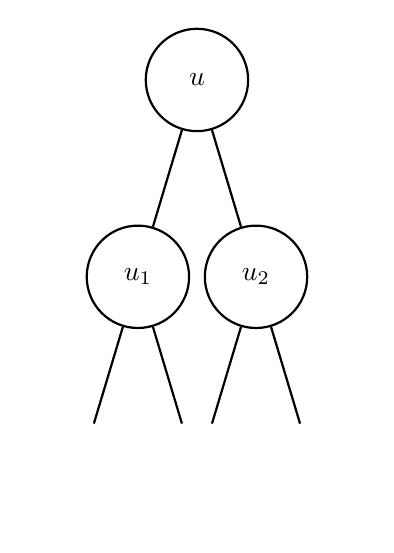
\begin{tikzpicture}[thick, minimum size=1.3cm, level distance=2.5cm]
    \node[circle,draw]{$u$}
        child { node[circle,draw]{$u_1$}
            child { node[circle]{}}
            child { node[circle]{}}
        }
        child { node[circle,draw]{$u_2$}
            child { node[circle]{}}
            child { node[circle]{}}
        };
  \end{tikzpicture}
  }
\end{center}
\caption{Binary tree starting at root r, branches below $u_1, u_2$ denotes subtrees}
\label{root_case}
\end{figure}

We begin by using that the root $u$ is independent of its children given $Z_u, Z_{u_1}, Z_{u_2}$ which leads to the following factorisation.
\begin{align}
  p(X) & = \sum_Z p(X,Z) = \sum_Z p(X_u, X_{u_1}, X_{u_2}, X_{u_1\downarrow}, X_{u_2\downarrow}, Z) \nonumber \\
  & = \sum_Z p(X_u, X_{u_1}, X_{u_2}, X_{u_1\downarrow}, X_{u_2\downarrow}, Z_{u_1\downarrow}, Z_{u_2\downarrow}| Z_u, Z_{u_1}, Z_{u_2})p(Z_u, Z_{u_1}, Z_{u_2}) \nonumber\\
  & = \sum_Z p(X_u|Z_{u_1}, Z_{u_2}, Z_u) p(Z_{u_1}, Z_{u_2}, Z_u)
  p(X_{u_1}, X_{u_1 \downarrow}, Z_{u_1 \downarrow}|Z_{u_1}, Z_u)
  p(X_{u_2}, X_{u_2 \downarrow}, Z_{u_2 \downarrow}|Z_{u_2}, Z_u) \nonumber\\
\end{align}
We can now let the sums over $Z_{u_1 \downarrow}$ and $Z_{u_2 \downarrow}$ move in which yields that
\begin{align}
  p(X) & = \sum_{Z_u, Z_{u_1}, Z_{u_2}}\bigg[p(X_u|Z_{u_1}, Z_{u_2}, Z_u) p(Z_{u_1}, Z_{u_2}, Z_u) \nonumber\\
  & \qquad\qquad\quad \Big(\sum_{Z_{u_1 \downarrow}} p(X_{u_1}, X_{u_1 \downarrow}, Z_{u_1 \downarrow}|Z_{u_1}, Z_u) \Big)\Big(\sum_{Z_{u_2 \downarrow}} p(X_{u_2}, X_{u_2 \downarrow}, Z_{u_2 \downarrow}|Z_{u_2}, Z_u) \Big)\bigg] \nonumber \\
\end{align}
Using that the latent variables $Z$ are independent given $\pi$ and substituting for the available densities yields
\begin{align}
  p(X) & = \sum_{Z_u, Z_{u_1}, Z_{u_2}}\bigg[\mathcal{N}\Big(X_u|(1-\alpha)\mu_{Z_u} +\frac{\alpha}{2}(\mu_{Z_{u_1}}+\mu_{Z_{u_2}}), \sigma^2 \Big) \pi(Z_u) \pi(Z_{u_1}) \pi(Z_{u_2})\\
  & \qquad\quad
  \Big(\underbrace{\sum_{Z_{u_1 \downarrow}} p(X_{u_1}, X_{u_1 \downarrow}, Z_{u_1 \downarrow}|Z_{u_1}, Z_u)}_\text{$p_{Z_{u_1 \downarrow}}$} \Big)
  \Big(\underbrace{\sum_{Z_{u_2 \downarrow}} p(X_{u_2}, X_{u_2 \downarrow}, Z_{u_2 \downarrow}|Z_{u_2}, Z_u)}_\text{$p_{Z_{u_2 \downarrow}}$} \Big) \bigg]
\end{align}
Where $p_{Z_{u_1 \downarrow}}$ and $p_{Z_{u_2 \downarrow}}$ denotes two independent subproblems with respect to the sets of latent variables $Z_{u_1 \downarrow}$ and $Z_{u_2 \downarrow}$

\subsection*{Starting at a node within the tree}
Now we will show how we can continue to divide each subproblem $p_{Z_{u_1 \downarrow}}$ and $p_{Z_{u_2 \downarrow}}$ defined above until the leaves are reached. We will now let $u_{1}$ and $u_{2}$ be the children of node $u$ and we will treat the problem shown in figure \ref{within_tree}


\begin{figure}[H]
\begin{center}
  \scalebox{0.7}{
  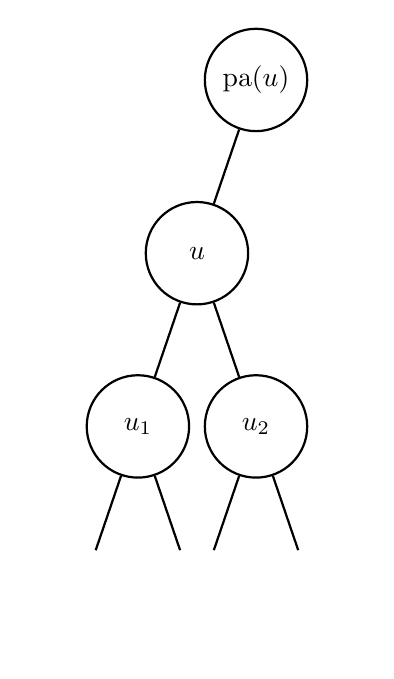
\begin{tikzpicture}[thick, minimum size=1.3cm, level distance=2.2cm]
    \node[circle,draw]{pa$(u)$}
        child { node[circle,draw]{$u$}
            child { node[circle,draw]{$u_1$}
                child { node[circle]{} }
                child { node[circle]{} }
                }
            child { node[circle,draw]{$u_2$}
                child { node[circle]{} }
                child { node[circle]{} }
                }
        }
        child [ missing ];
  \end{tikzpicture}
  }
\end{center}
  \caption{Binary tree starting at parent of $u$, branches below $u_1, u_2$ denotes subtrees}
  \label{within_tree}
\end{figure}

Let $p_{Z_{u \downarrow}} = \sum_{Z_{u \downarrow}} p(X_u, X_{u \downarrow}, Z_{u \downarrow}|Z_u, Z_{\text{pa}(u)})$, then

\begin{align}
  p_{Z_{u \downarrow}} & = \sum_{Z_{u \downarrow}} p(X_u, X_{u_1}, X_{u_2}, X_{u_1 \downarrow}, X_{u_2 \downarrow}, Z_{u_1 \downarrow}, Z_{u_2 \downarrow}|Z_u, Z_{\text{pa}(u)}, Z_{u_1}, Z_{u_2})p(Z_{u_1}) p(Z_{u_1\downarrow}) \nonumber \\
  & = \sum_{Z_{u \downarrow}} p(X_u|Z_u, Z_{\text{pa}(u)}, Z_{u_1}, Z_{u_2}) p(Z_{u_1})p(Z_{u_2})p(X_{u_1}, X_{u_1\downarrow}, Z_{u_1\downarrow}|Z_{u_1}, Z_u) p(X_{u_2}, X_{u_2\downarrow}, Z_{u_2\downarrow}|Z_{u_2}, Z_u) \nonumber\\
  & = \sum_{Z_{u \downarrow}} \bigg[ p(X_u|Z_u, Z_{\text{pa}(u)}, Z_{u_1}, Z_{u_2})p(Z_{u_1})p(Z_{u_2}) \nonumber\\
  & \qquad\qquad p(X_{u_1}, X_{u_1\downarrow}, Z_{u_1\downarrow}|Z_{u_1}, Z_u) p(X_{u_2}, X_{u_2\downarrow}, Z_{u_2\downarrow}|Z_{u_2}, Z_u) \bigg] \nonumber\\
  & = \sum_{Z_{u_1}, Z_{u_2}} \bigg[ p(X_u|Z_u, Z_{\text{pa}(u)}, Z_{u_1}, Z_{u_2})p(Z_{u_1})p(Z_{u_2}) \nonumber\\
  & \qquad\qquad
  \Big( \sum_{Z_{u_1\downarrow}} p(X_{u_1}, X_{u_1\downarrow}, Z_{u_1\downarrow}|Z_{u_1}, Z_u) \Big)
  \Big( \sum_{Z_{u_2\downarrow}} p(X_{u_2}, X_{u_2\downarrow}, Z_{u_2\downarrow}|Z_{u_2}, Z_u)\Big) \bigg] \nonumber\\
  & = \sum_{Z_{u_1}, Z_{u_2}} \bigg[ p(X_u|Z_u, Z_{\text{pa}(u)}, Z_{u_1}, Z_{u_2})p(Z_{u_1})p(Z_{u_2}) \Big(p_{Z_{u_1\downarrow}}\Big) \Big( p_{Z_{u_2\downarrow}}\Big)\bigg] \nonumber \\
  & = \sum_{Z_{u_1}, Z_{u_2}} \bigg[ \mathcal{N}\Big(X_u|(1-\alpha)\mu_{Z_u} +\frac{\alpha}{3}(\mu_{Z_{u_1}}+\mu_{Z_{u_2}}+\mu_{Z_{\text{pa}(u)}}), \sigma^2 \Big) \cdot \nonumber\\
  & \qquad\qquad\qquad  \cdot \pi(Z_{u_1}) \pi(Z_{u_2}) \Big(p_{Z_{u_1\downarrow}}\Big) \Big( p_{Z_{u_2\downarrow}}\Big)\bigg]\nonumber
\end{align}

On a more compact form we have thus shown that

\begin{align}
  p_{Z_{u \downarrow}} & = \sum_{Z_{u \downarrow}} p(X_u, X_{u \downarrow}, Z_{u \downarrow}|Z_u, Z_{\text{pa}(u)}) \\
  & = \sum_{Z_{u_1}, Z_{u_2}} \bigg[ \mathcal{N}\Big(X_u|(1-\alpha)\mu_{Z_u} +\frac{\alpha}{3}(\mu_{Z_{u_1}}+\mu_{Z_{u_2}}+\mu_{Z_{\text{pa}(u)}}), \sigma^2 \Big) \cdot \label{rec1}\\
  & \qquad\qquad\qquad  \cdot \pi(Z_{u_1}) \pi(Z_{u_2}) \Big(p_{Z_{u_1\downarrow}}\Big) \Big( p_{Z_{u_2\downarrow}}\Big)\bigg] \label{rec2}
\end{align}
Which shows the recursion.


We have thus ended up with two new subproblems $p_{Z_{u_1\downarrow}}$ and $p_{Z_{u_2\downarrow}}$ from $p_{Z_{u \downarrow}}$ which can be divided into subproblems continuously until the leaves are reached.
\\

It is important to note that $p_{Z_{u_1\downarrow}}$ is independent of $Z_{u_2}$ and similarly $p_{Z_{u_2\downarrow}}$ is independent of $Z_{u_1}$. It is thus only necessary to compute $p_{Z_{u_1\downarrow}}$ when summing over $Z_{u_1}$. When summing over $Z_{u_2}$ the value for $p_{Z_{u_1\downarrow}}$ can be computed once, stored and then be reused. Applying this for all subproblems results in a linear algorithm for computing $p(X)$.


\subsection*{Starting at a leaf}
When equation \eqref{rec1} $+$ \eqref{rec2} has been used recursively until the leaves are reached we need to show that the DP-algorithm can be started there. Let $u_1$ denote a \textit{leaf node}, it thus has no children which implies that $Z_{u_1 \downarrow} = \emptyset$. Using previous definition of $p_{Z_{u \downarrow}}$ yields

 \begin{align}
   p_{Z_{u_1 \downarrow}} & = \sum_{Z_{u_1 \downarrow}} p(X_{u_1}, X_{u_1 \downarrow}, Z_{u_1 \downarrow}|Z_{u_1}, Z_{\text{pa}(u_1)}) \nonumber\\
   & = p(X_{u_1}|Z_{u_1}, Z_{\text{pa}(u_1)}) \nonumber\\
   & = \mathcal{N}\Big(X_{u_1} | (1-\alpha)\mu_{Z_{u_1}} + \alpha \mu_{Z_{\text{pa}(u_1)}}, \sigma^2 \Big)
 \end{align}
